\section{Results: The Controlled Grid}
\label{sec:results-controlled-grid}

% src: docs/results_of_record/controlled_grid_2026_10/{centre_bs,ne_bs}/results_summary.csv (regenerated 2026-10-13); technical_documentation.md §7.2.1, §7.3.2; constant-guess MAE 10.9 m from the test portion of the centre-BS data
Without AoA, adding three steps of history to RSS and SINR raised exact-cell accuracy in every configuration of the controlled-grid study, for both classifiers and both BS placements~(Figure~\ref{fig:cg-placement}). With the BS at the center, XGBoost gained $14.4$ percentage points ($13.8\%$ to $28.2\%$) and Random Forest $11.7$ ($22.7\%$ to $34.3\%$); with the BS beyond the corner they gained $13.3$ ($11.3\%$ to $24.7\%$) and $9.7$ points ($18.8\%$ to $28.5\%$). Mean position error fell by $2.5$ to $3.2\,\text{m}$ in all four cases, between $27\%$ and $33\%$. These snapshot models are weak: always guessing the center of the grid gives a mean error of $10.9\,\text{m}$ on the test samples, and without history XGBoost reaches $10.4\,\text{m}$ and Random Forest $9.2\,\text{m}$ at the center. History therefore lifts RSS and SINR from a level close to the trivial guess to a modest one, and the gain is of similar size for both classifiers and both placements.

\begin{figure}[h]
  \centering
  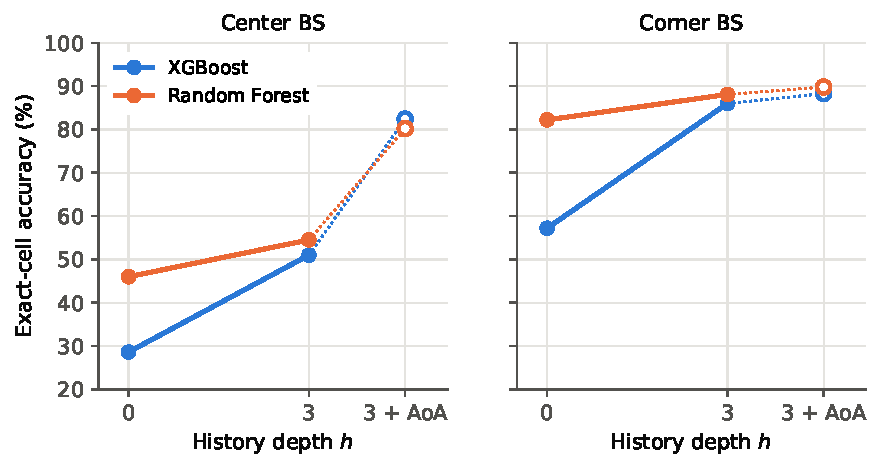
\includegraphics[width=0.85\textwidth]{fig_controlled_grid_placement}
  \caption{Controlled grid: exact-cell accuracy from RSS and SINR, and with AoA added, at history depth $h=0$ and $h=3$, with the BS at the grid center~(left) and beyond its corner~(right). Single run per configuration, simulated at $3.5\,\text{GHz}$ with one urban-micro NLOS propagation scenario for every walk.}
  \label{fig:cg-placement}
\end{figure}
% src: technical_documentation.md §7.2.1, §7.3.1, §7.3.3; figure_scripts/make_figures.py controlled_grid_placement()

% src: results_of_record/controlled_grid_2026_10 results_summary.csv (BASE_H3 vs BASE_A_H3); technical_documentation.md §7.3.1
The same placement change that leaves history's contribution positive removes most of AoA's. With history already in the input, adding AoA raised XGBoost's accuracy by $39.2$ points at the center BS but by $6.2$ points at the corner, and Random Forest's by $33.0$ and $5.8$ points. From the corner the whole grid falls within a wedge of about $52^\circ$, and once a $5^\circ$ codebook and a few degrees of estimation noise are applied, azimuth no longer separates neighboring cells; with AoA and history the corner placement reaches only $30.9\%$ for XGBoost against $67.5\%$ at the center. The remaining gain at the corner is consistent with elevation, which encodes distance, but this grid study does not isolate it. This loss of AoA's value is specific to a short-range grid with $2\,\text{m}$ cells; it is not a general property of corner placements.

% src: FINDINGS.md §3.3 (7x7, RSS+SINR, raw stacking: XGB 26.8/38.7/43.5/45.4; RF 28.0/38.3/42.6/43.6; MLP 24.8/36.9/38.6/41.6); analysis/regression_vs_classification.md §4.1-4.2 (15x15 single scenario with AoA: UMa NLOS 29.18/46.12/49.48/51.23; UMa LOS 92.59/95.90/95.54/95.86)
Where history was swept one step at a time, most of the gain arrived with the first step~(Figure~\ref{fig:cg-depth}). On a single-user $7\times7$ grid, one step of history raised accuracy by $10$ to $12$ points for each of XGBoost, Random Forest and a multilayer perceptron, and the next two steps added about $5$ to $7$ points between them. With AoA available, the same profile appears in a uniform urban-macro NLOS scenario, where accuracy rose from $29\%$ to $46\%$ at the first step and to $51\%$ by $h=3$. In the corresponding LOS scenario, where AoA alone already placed $93\%$ of samples in the right cell, history added $3$ points at the first step and nothing after it.

\begin{figure}[h]
  \centering
  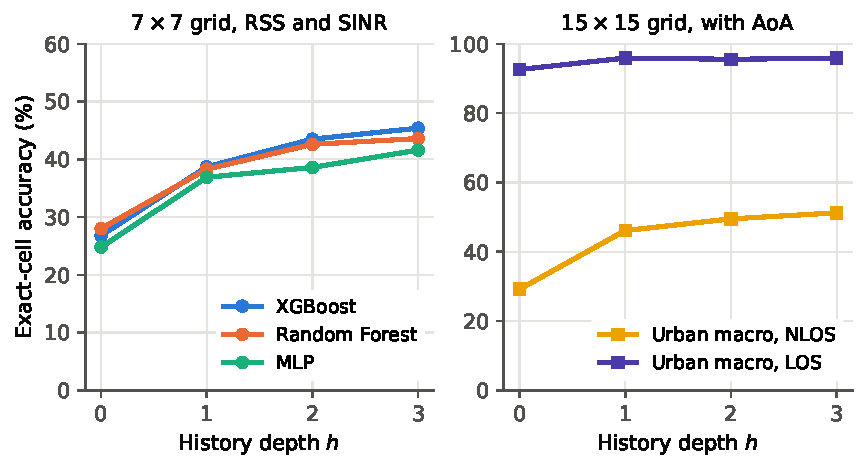
\includegraphics[width=0.85\textwidth]{fig_controlled_grid_depth}
  \caption{Controlled grid, single user: exact-cell accuracy as history depth grows. Left: $7\times7$ grid with RSS and SINR, three classifiers. Right: $15\times15$ grid with AoA in a single urban-macro propagation scenario, NLOS and LOS. Single run per point.}
  \label{fig:cg-depth}
\end{figure}
% src: figure_scripts/make_figures.py controlled_grid_depth()

% src: technical_documentation.md §7.1 (grid sweep, single user, XGBoost); §7.1 second table (7x7, four algorithms)
The direction of the history effect is also stable across scale and estimator~(Figure~\ref{fig:cg-scale}). In the single-user version of the study, history raised accuracy at every grid size from $3\times3$ to $20\times20$ cells, by between $9.2$ and $21.8$ points, and on the $7\times7$ grid it raised the accuracy of all four estimators tried, from $4.7$ points for a Gaussian likelihood model to $18.2$ points for XGBoost.

\begin{figure}[h]
  \centering
  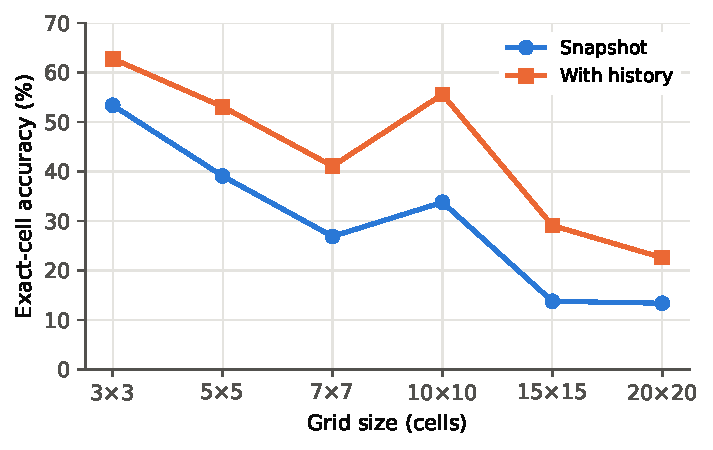
\includegraphics[width=0.65\textwidth]{fig_controlled_grid_scale}
  \caption{Controlled grid, single user: exact-cell accuracy with and without history as the grid grows from $3\times3$ to $20\times20$ cells, XGBoost with RSS and SINR at the best depth up to $h=3$. Single run per grid size.}
  \label{fig:cg-scale}
\end{figure}
% src: technical_documentation.md §7.1; figure_scripts/make_figures.py controlled_grid_scale()

% src: results_of_record/controlled_grid_2026_10/centre_bs/results_summary.csv (BASE_dp 25.88/30.58 -> BASE_H3_dp 33.75/39.72; BASE_A_dp 65.41/67.26 -> BASE_A_H3_dp 68.42/67.85); technical_documentation.md §7.2.6
Because RSS and SINR are stacked in absolute form, part of what a history window carries is a stable, device-specific offset, and history could in principle be helping only by identifying the device. Supplying the device parameters directly rules this out as the whole story: with antenna count, gain and height already in the input, history still added $7.9$ points for XGBoost and $9.1$ for Random Forest at the center BS. The device parameters themselves are worth about as much as history ($12.0$ and $7.9$ points over the snapshot model), and the user identifier alone is as informative as the parameters, so their gain is a device-identity effect. With AoA available at the center BS, history added less, $3.0$ points for XGBoost and $0.6$ for Random Forest on top of the device parameters, since a classifier that already reaches about $65\%$ from AoA has less ambiguity left for history to resolve.

% src: earlier pair of runs of the same configuration (technical_documentation.md history; superseded data) differed by 2-3 points; the controlled-grid runs were regenerated 2026-10-13 (RESULTS_DIRECTORY_MAP.md §7)
Every number in this section comes from a single run, and the same configuration evaluated in two separate runs differed by $2$ to $3$ points in an earlier version of this study, so only differences well above that are read as effects. The depth and scale sweeps above come from earlier single-user simulations that were not regenerated. The controlled grid also tests later time steps of users seen in training, at no more than $61\,\text{m}$ from the BS. Whether history keeps its value at macro-cell range, for users the model has never seen and a population with mixed hardware, is the question the macro-cell study answers.
